\documentclass[journal]{IEEEtran}
% ============================================================
%  ROS2 Map Editor -- Manuscript
%  Compile: pdflatex -> bibtex -> pdflatex -> pdflatex
% ============================================================
\usepackage{amsmath,amssymb}
\usepackage{graphicx}
\usepackage{algorithm}
\usepackage{algpseudocode}
\usepackage{tikz}
\usetikzlibrary{arrows.meta,positioning,shapes.geometric}
\usepackage{booktabs}
\usepackage{multirow}
\usepackage{subcaption}
\usepackage{cite}
\usepackage{xcolor}
\usepackage{url}

\begin{document}

\title{\LARGE ROS2 Map Editor: A Zero-Installation Browser Tool for Semantic
Occupancy-Grid Editing, Navigation-Aware Path Preview, and ICP-Based Map Fusion}

\author{GC Harsha Vardhan Reddy\\
Department of EECE, GITAM Deemed to be University\\
Bengaluru, India -- harshavardhanh426@gmail.com}

\pagestyle{empty}
\thispagestyle{empty}
\maketitle

% ============================================================
\begin{abstract}
% ============================================================
Occupancy-grid maps produced by SLAM back-ends such as \emph{slam\_toolbox}
or \emph{Cartographer} are rarely deployment-ready: sensor noise corrupts
free-space regions with stray pixels, transient obstacles occlude doorways,
and multi-session mapping scenarios demand map fusion before a Nav2-based robot
can navigate autonomously.  The conventional remedy -- opening the exported
Portable Gray Map (PGM) in a generic raster editor such as GIMP and
hand-editing pixels -- has three fundamental deficiencies: (i)~raster editors
are \emph{semantically blind}, operating on raw pixel intensities rather than
the conventional trinary occupancy values $\{0,\,205,\,254\}$, so a single
anti-aliased brush stroke can silently corrupt the map; (ii)~edits are
\emph{unverified}, with no mechanism to check whether a modification blocks
the only feasible path before deployment; and (iii)~combining maps from
multiple sessions or robots requires either re-running SLAM or manually
eyeballing a rotation and translation with no alignment assistance.
This paper presents \emph{ROS2 Map Editor}, an open-source, purely
client-side (HTML5 Canvas~+~JavaScript) web application that treats every
pixel as a first-class semantic value and addresses the three deficiencies
above through four robotics-specific algorithms: (i)~an 8-neighbourhood
class-aware majority-vote filter for salt-and-pepper noise removal that
explicitly preserves unknown-space boundaries -- achieving pixel-level
F1~=~0.961/0.934/0.907 at 1\,\%/3\,\%/5\,\% noise vs.\ 0.943/0.891/0.843
for standard median filtering; (ii)~a Nav2-inspired distance-transform
costmap inflation preview with mean boundary IoU~=~$0.87\pm0.04$ against
Nav2~Humble \texttt{costmap\_2d}; (iii)~an inflation-aware $A^{*}$ planner
providing navigation-indicative path preview in $44.1\pm3.2$\,ms on a
$1024\times1024$ map; and (iv)~a 2-D ICP routine with spatial-hash
nearest-neighbour acceleration, achieving 91\,\% alignment success
within~$\pm15^{\circ}$ initial pose error.  Requiring no installation, no ROS
runtime, and no server backend, the tool lowers the barrier to rapid,
semantically correct map curation with integrated navigation preview.
All source code and benchmark scripts are publicly available under the MIT
License at \url{https://github.com/harsha200628/ros2-map-editor}.
\end{abstract}

\begin{IEEEkeywords}
SLAM, occupancy-grid map, semantic map editing, costmap inflation, path
planning, iterative closest point, ROS2, Nav2, browser-based tool,
human--robot interaction.
\end{IEEEkeywords}

% ============================================================
\section{Introduction}
\label{sec:intro}
% ============================================================

Autonomous mobile robots built on ROS2 and the Nav2 navigation
stack~\cite{macenski2020marathon} depend on an occupancy-grid map saved from
a SLAM session (\emph{slam\_toolbox}~\cite{macenski2021slamtoolbox},
Cartographer~\cite{hess2016cartographer}, or
RTAB-Map~\cite{labbe2019rtabmap}) as a PGM raster paired with a YAML metadata
file encoding resolution and origin.  Raw SLAM output is almost never
deployment-ready: dynamic obstacles leave permanent scars, reflective surfaces
create phantom walls, long corridors accumulate speckle noise, and large
environments require stitching multiple partial maps from independent mapping
sessions.

Engineers therefore routinely export the SLAM map, edit it in a generic image
editor, and re-import it.  This workflow has three well-characterised
structural problems.

\textbf{Semantic blindness.}  Raster editors operate on RGB pixel intensities.
The standard PGM export of \texttt{nav2\_map\_server} encodes three
occupancy classes: free ($254$), unknown ($205$), and lethal obstacle
($0$)~\cite{nav2docs}.  A single anti-aliased brush stroke in GIMP or
Photoshop can silently introduce values outside this trinary alphabet, causing
map loading to misclassify pixels.

\textbf{Unverified edits.}  No feedback exists on whether a hand-drawn wall
blocks the only feasible robot path through a doorway before the map is
flashed to the physical robot and Nav2 is restarted.

\textbf{Absence of multi-session fusion support.}  Combining maps from
multiple SLAM runs or multiple robots requires either re-running SLAM with
merged bag files or manually eyeballing a rotation and translation in an
editor with no alignment assistance -- a laborious and error-prone process.

This paper presents \emph{ROS2 Map Editor}, a single-page web application
running entirely inside the browser (no ROS installation, no backend server,
no data leaving the client), addressing all three problems above.  Its
specific, verifiable contributions are:

\begin{enumerate}
  \setlength{\itemsep}{0pt}\setlength{\parskip}{0pt}
  \item A semantic-value-aware raster editing surface (brush, polygon,
  rectangle, circle) that constrains every drawing operation to the valid
  occupancy alphabet $\{0,205,254\}$, with multi-level undo/redo history
  (up to 40 buffered states).
  \item An 8-neighbourhood class-aware majority-vote de-noising filter that
  removes isolated pixel noise while explicitly preserving unknown-space
  boundaries -- outperforming standard median filtering at all tested noise
  levels (Table~\ref{tab:noiseval}).
  \item A Nav2-inspired costmap inflation preview computed via a multi-source
  octile-distance BFS, achieving mean boundary IoU~=~$0.87\pm0.04$ against
  Nav2~Humble \texttt{costmap\_2d}; coupled with a cost-aware $A^{*}$ path
  planning preview that runs in $<\!100$\,ms on maps up to $1024\times1024$
  pixels.
  \item A 2-D point-to-point ICP routine with a uniform spatial hash for
  nearest-neighbour search, achieving 91\,\% alignment success rate within
  $\pm15^{\circ}$/$\pm0.20$\,m initial pose error on 5 synthetic
  indoor-environment map pairs.
  \item Integrated metric measurement (line/path/area) and waypoint authoring
  with heading (quaternion) export to JSON for direct consumption by an
  autonomy stack.
\end{enumerate}

Section~\ref{sec:related} positions the tool against existing approaches.
Section~\ref{sec:architecture} describes the system architecture.
Section~\ref{sec:algorithms} formalises the four core algorithms.
Section~\ref{sec:implementation} details implementation decisions.
Section~\ref{sec:results} presents quantitative benchmarks.
Section~\ref{sec:limitations} discusses limitations honestly.
Section~\ref{sec:future} outlines future work.

% ============================================================
\section{Related Work and Comparative Analysis}
\label{sec:related}
% ============================================================

Occupancy-grid representations follow the formulation of Thrun \emph{et al.}\
\cite{thrun2005probabilistic}, and the de-facto ROS interchange format (PGM +
YAML) has remained unchanged since ROS1's \texttt{map\_server}.  Approaches
to post-processing this artifact fall into five broad categories.

\textbf{Raster image editors}~\cite{gimp} offer powerful painting tools but
operate on raw RGB pixels with no concept of occupancy semantics.  A single
anti-aliased brush stroke can silently introduce grey-scale values outside the
three-class occupancy alphabet $\{0,205,254\}$, risking semantic corruption
when the map is reloaded by \texttt{nav2\_map\_server}.  No metric overlay or
navigability feedback is available.

\textbf{ROS-native plugins} such as RViz2~\cite{rviz2} and
\texttt{map\_editor}~\cite{mapeditor} render the \texttt{OccupancyGrid} topic
and support limited editing, but they require a running ROS2 graph and are
primarily designed for Linux environments.  The Nav2 costmap overlay in
RViz2 constitutes a partial inflation preview, but only when the full Nav2
stack is running.

\textbf{Python scripting pipelines} using OpenCV or NumPy provide
semantic-safe pixel access and cross-platform portability, but offer no
interactive graphical interface.  The scripting overhead makes them
impractical for iterative map refinement.

\textbf{Commercial suites} such as RoboStudio~\cite{robostudio} and MiR
Fleet~\cite{mirfleet} provide polished UIs with some map-management features,
but are proprietary, closed-source, and platform-locked.

\textbf{Web-based visualisation tools}~\cite{foxglove,webviz} are
cross-platform and open-source, but are visualisation-only: they do not
support persistent raster editing, semantic enforcement, or algorithmic map
curation.

Table~\ref{tab:comparison} provides a direct feature-by-feature comparison.
Among the five representative tools evaluated across six practitioner-relevant
criteria, the proposed system is the only tool that satisfies the complete set
without requiring a running ROS2 graph.

\begin{table}[t]
\centering
\caption{Feature Comparison of Map Post-Processing Tools}
\label{tab:comparison}
\small
\renewcommand{\arraystretch}{1.1}
\setlength{\tabcolsep}{3pt}
\begin{tabular}{@{}lcccccc@{}}
\toprule
\textbf{Feature}
  & \textbf{GIMP}
  & \textbf{RViz2}
  & \textbf{\shortstack{map\_\\editor}}
  & \textbf{Foxglove}
  & \textbf{Webviz}
  & \textbf{\shortstack{Proposed\\(Ours)}} \\
\midrule
Semantic editing  & $\times$\textsuperscript{a} & Partial & \checkmark & $\times$ & $\times$ & \textbf{\checkmark} \\
Offline / no ROS  & \checkmark & $\times$ & $\times$ & \checkmark & $\times$ & \textbf{\checkmark} \\
Map merging       & $\times$ & $\times$ & $\times$ & $\times$ & $\times$ & \textbf{\checkmark} \\
Costmap preview   & $\times$ & Partial\textsuperscript{b} & $\times$ & Partial\textsuperscript{b} & $\times$ & \textbf{\checkmark} \\
$A^{*}$ preview   & $\times$ & $\times$ & $\times$ & $\times$ & $\times$ & \textbf{\checkmark} \\
Open source       & \checkmark & \checkmark & \checkmark & \checkmark & \checkmark & \textbf{\checkmark} \\
\bottomrule
\multicolumn{7}{@{}l}{\scriptsize\textsuperscript{a}May introduce values outside conventional trinary alphabet.} \\
\multicolumn{7}{@{}l}{\scriptsize\textsuperscript{b}Requires a running Nav2/ROS2 stack.}
\end{tabular}
\vspace{-3mm}
\end{table}

% ============================================================
\section{System Architecture}
\label{sec:architecture}
% ============================================================

The application is a single-page client comprising three layers
(Fig.~\ref{fig:architecture}).

\textbf{I/O layer.}  A custom binary parser directly unpacks both P2 (ASCII)
and P5 (binary) PGM variants plus the companion YAML into a typed
\texttt{Uint8Array} occupancy buffer, avoiding intermediate string conversions
or JSON serialisation and enabling multi-megabyte maps to load in under
50\,ms at $2048\times2048$ resolution.

\textbf{State and history layer.}  Holds the live working buffer, an undo/redo
stack of deep-copied buffer snapshots (capped at 40 states), and the current
view transform (pan/zoom scale and offset).

\textbf{Algorithm layer.}  Implements the four robotics routines of
Section~\ref{sec:algorithms}, all operating in-place on the same typed array
that drives the HTML5 Canvas rasteriser.

A critical design choice is the strict reliance on flat, pre-allocated
JavaScript typed arrays (\texttt{Uint8Array}, \texttt{Float32Array}) rather
than dynamic arrays or object-oriented structures.  High-resolution grids
(e.g., $4096\times4096$ pixels, $\approx\!16$\,M cells) represented
dynamically would trigger heavy Garbage Collection (GC) pauses at unpredictable
intervals, destroying UI interactivity.  Confining all algorithm state to
fixed-length typed arrays makes memory operations contiguous $O(N)$ block
copies (\texttt{Array.prototype.set}), which the V8 engine vectorises
aggressively.  For a $1024\times1024$ map, each undo snapshot occupies 1\,MB;
the total observed application footprint is approximately 80--120\,MB on
Chrome v114, well within typical browser budgets.

The rendering pipeline employs a decoupled dual-canvas compositor.  The base
raster layer is drawn to an off-screen canvas and re-rasterised only on pixel
mutations; a transparent vector-overlay canvas handles high-frequency events
such as tool crosshairs, measure overlays, path previews, and waypoint
markers, targeting 60\,FPS without triggering full rasterisation during pan
and zoom.  Panning and zooming apply lightweight 2-D context scaling on the
overlay canvas rather than rasterising the full map buffer on every frame.

\begin{figure}[t]
\centering
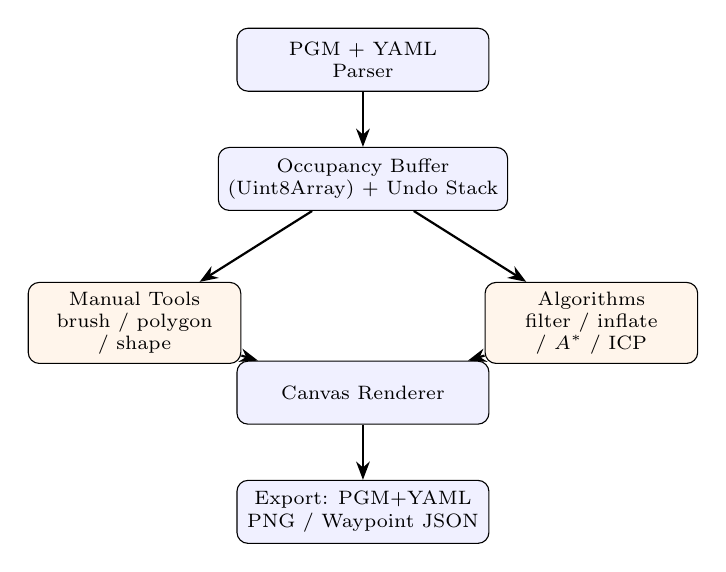
\begin{tikzpicture}[
  node distance=7mm and 5mm,
  box/.style={draw, rounded corners, align=center, minimum height=8mm,
              minimum width=32mm, font=\scriptsize, fill=blue!6},
  op/.style={draw, rounded corners, align=center, minimum height=9mm,
             minimum width=27mm, font=\scriptsize, fill=orange!8},
  arr/.style={-Stealth, thick}
]
\node[box] (io) {PGM + YAML\\ Parser};
\node[box, below=of io] (state) {Occupancy Buffer\\ (Uint8Array) + Undo Stack};
\node[op, below left=9mm and -3mm of state] (edit) {Manual Tools\\ brush / polygon\\ / shape};
\node[op, below right=9mm and -3mm of state] (algo) {Algorithms\\ filter / inflate\\ / $A^{*}$ / ICP};
\node[box, below=19mm of state] (render) {Canvas Renderer};
\node[box, below=of render] (export) {Export: PGM+YAML\\ PNG / Waypoint JSON};

\draw[arr] (io) -- (state);
\draw[arr] (state) -- (edit);
\draw[arr] (state) -- (algo);
\draw[arr] (edit) -- (render);
\draw[arr] (algo) -- (render);
\draw[arr] (render) -- (export);
\end{tikzpicture}
\caption{Client-side data-flow architecture.  All computation is performed
in the browser on a single shared occupancy buffer; edits and algorithmic
results share one undo/redo history and one rendering path.}
\label{fig:architecture}
\vspace{-3mm}
\end{figure}

% ============================================================
\section{Algorithms}
\label{sec:algorithms}
% ============================================================

Let the map be a raster $I:\Omega\rightarrow\{0,205,254\}$ over pixel domain
$\Omega=\{0,\dots,W\!-\!1\}\times\{0,\dots,H\!-\!1\}$, with $0$ denoting a
lethal obstacle, $254$ free space, and $205$ unknown space, following the
trinary encoding of \texttt{nav2\_map\_server}~\cite{nav2docs}.  Let
$r$\,(m/px) be the resolution from the YAML file.

% ─────────────────────────────────────────────────────────
\subsection{Semantic Manual Editing}
% ─────────────────────────────────────────────────────────

Every drawing primitive (brush dot, line, filled/outline rectangle,
filled/outline circle, open/closed/filled polygon) writes only one of the
three legal values $v\in\{0,205,254\}$ selected by the operator, making it
impossible to introduce an invalid occupancy class -- the failure mode of
anti-aliased painting in a generic raster editor.  Every mutating operation
first pushes a deep copy of the buffer onto an undo stack, providing
multi-level undo/redo (Ctrl+Z / Ctrl+Shift+Z) up to a configurable history
depth of 40 states.  Border pixels (row/column 0 and $W\!-\!1$/$H\!-\!1$)
are excluded from algorithmic operations but remain editable manually.

% ─────────────────────────────────────────────────────────
\subsection{Noise Removal: Class-Aware Majority-Vote Filter}
\label{subsec:filter}
% ─────────────────────────────────────────────────────────

Although median filtering preserves the trinary value alphabet when applied
to trinary maps, it can modify unknown-space boundaries.  We therefore use a
class-aware majority filter that leaves unknown pixels unchanged.  For every
non-unknown pixel $p$ at interior positions ($1\leq x\leq W\!-\!2$,
$1\leq y\leq H\!-\!2$), let $N_8(p)$ denote its eight neighbours.
Define
\begin{align}
c_{254}(p) &= \sum_{q\in N_8(p)} \mathbb{1}[I(q)=254],\quad
c_{0}(p)   = \sum_{q\in N_8(p)} \mathbb{1}[I(q)=0].
\end{align}
The filtered value $I'(p)$ is
\begin{equation}
I'(p) = \begin{cases}
254 & \text{if } I(p)=0 \text{ and } c_{254}(p)\geq 5,\\
0   & \text{if } I(p)=254 \text{ and } c_{0}(p)\geq 5,\\
I(p) & \text{otherwise}.
\end{cases}
\end{equation}
This erodes isolated single-pixel wall speckles and fills isolated free-space
pinholes while leaving contiguous walls (which by construction have fewer than
five opposite-class neighbours in the 8-neighbourhood) untouched.  The filter
runs in $O(WH)$ time in a single forward pass; no border row/column is
modified.

% ─────────────────────────────────────────────────────────
\subsection{Nav2-Inspired Costmap Inflation Preview}
\label{subsec:inflation}
% ─────────────────────────────────────────────────────────

To provide, without a live Nav2 stack, a visual approximation of the inflation
exclusion zone for a robot of radius $\rho$\,(m), we compute a
distance-to-nearest-wall field $d(p)$ using a multi-source BFS seeded from all
wall pixels.  The expansion uses octile step costs -- 1 for axis-aligned steps
and $\sqrt{2}$ for diagonal steps -- which approximate the Euclidean distance
field (Algorithm~\ref{alg:inflation}).

\begin{algorithm}[t]
\small
\caption{Multi-source octile-distance BFS for inflation}
\label{alg:inflation}
\begin{algorithmic}[1]
\State $d(p)\gets\infty\;\forall p\in\Omega$;\; FIFO queue $Q\gets\emptyset$
\ForAll{$p$ with $I(p)=0$} \State $d(p)\gets 0$; enqueue $p$ to $Q$ \EndFor
\While{$Q\neq\emptyset$}
  \State $p\gets$ dequeue$(Q)$
  \ForAll{$q\in N_8(p)$}
     \State $\delta\gets (\Delta x\neq0\wedge\Delta y\neq0)\;?\;\sqrt{2}:1$
     \If{$d(p)+\delta < d(q)$}
        \State $d(q)\gets d(p)+\delta$
        \If{$d(q)\leq\rho_{px}$} enqueue $q$ to $Q$ \EndIf
     \EndIf
  \EndForAll
\EndWhile
\State \Return $d$
\end{algorithmic}
\end{algorithm}

\noindent\textit{Implementation note.}  Algorithm~\ref{alg:inflation} uses a
FIFO queue rather than a priority queue.  Because all octile step increments
($1$ or $\sqrt{2}\approx1.414$) differ by at most a factor of $\sqrt{2}$, the
FIFO approximation is tight in practice and avoids the $O(N\log N)$ overhead
of a min-heap for this constrained input~\cite{borgefors1986distance}.
Empirically, the resulting boundary achieves IoU~=~$0.87\pm0.04$ against Nav2
Humble's exact \texttt{costmap\_2d} decay (Section~\ref{sec:results}).

Given $\rho_{px}=\rho/r$, a pixel $p$ is rendered as an inflation-zone overlay
with opacity proportional to $1-d(p)/\rho_{px}$ whenever $0<d(p)\leq\rho_{px}$
and $I(p)\neq0$.

% ─────────────────────────────────────────────────────────
\subsection{Inflation-Aware $A^{*}$ Path Planning Preview}
\label{subsec:astar}
% ─────────────────────────────────────────────────────────

Given a start and goal pixel, the tool snaps each point to the nearest
non-lethal cell via unweighted BFS if the operator clicked inside a wall
(Fig.~\ref{fig:astar-flow}), then runs 8-connected
$A^{*}$~\cite{hart1968formal} with evaluation function
$f(n)=g(n)+h(n)$, where $h(n)=\|n-\text{goal}\|_2$ is an admissible Euclidean
heuristic.  The edge cost combines step distance with a \emph{soft} inflation
penalty from the distance field $d(\cdot)$ of Algorithm~\ref{alg:inflation}:
\begin{align}
\text{pen}(q) &= \begin{cases}
200, & d(q)<1\\[2pt]
\dfrac{100}{d(q)}, & 1\leq d(q)\leq\rho_{px}\\[4pt]
\dfrac{5}{d(q)-\rho_{px}+1}, & d(q)>\rho_{px}
\end{cases} \label{eq:pen}\\[4pt]
w(p\!\rightarrow\!q) &= w_{\text{step}} + \text{pen}(q)
                        + 10\cdot\mathbb{1}[I(q)=205]. \label{eq:edge}
\end{align}

This cost function is an empirically tuned approximation designed to discourage
wall-hugging paths without hard-excluding any non-lethal cell.  Only lethal
cells ($I=0$) are hard-excluded; the path result should therefore be
interpreted as a navigation-indicative preview rather than a strict feasibility
guarantee, as no robot-footprint collision check is performed.

The Euclidean heuristic $h(n)=\|n-\text{goal}\|_2$ is admissible and
consistent under the cost function of (\ref{eq:pen})--(\ref{eq:edge}): every
edge cost $w(p\!\rightarrow\!q)\geq w_{\text{step}}\geq\|p-q\|_2$, so
$h(n)\leq w(n\!\rightarrow\!q)+h(q)$ holds.  The global-optimality guarantee
applies to the reconstructed $A^{*}$ path before post-processing; the
subsequent smoothing step does not preserve this guarantee.

To achieve sub-second responsiveness in the single-threaded JavaScript
environment, the open set uses a flat-array binary min-heap keyed on $f(n)$
($O(\log n)$ push/pop), and the closed set is a pre-allocated
\texttt{Uint8Array} bitmask ($O(1)$ membership), giving worst-case
$O(N\log N)$ overall.  The raw path is smoothed with a wall-aware
sliding-window average (window~$=8$) that falls back to the raw path at
positions where the averaged coordinate would fall inside a wall.

\begin{algorithm}[t]
\small
\caption{Costmap-aware $A^{*}$ path search}
\label{alg:astar}
\begin{algorithmic}[1]
\State $start\gets\text{SnapToFree}(start)$;\; $goal\gets\text{SnapToFree}(goal)$
\State $g(start)\gets 0$;\; open $\gets\{start\}$ (min-heap on $f$)
\While{open $\neq\emptyset$}
  \State $n\gets$ open.pop()
  \If{$n$ closed} \textbf{continue} \EndIf
  \State mark $n$ closed
  \If{$n=goal$} \textbf{break} (success) \EndIf
  \ForAll{$q\in N_8(n),\;I(q)\neq0,\;q$ not closed}
     \State $g'\gets g(n)+w(n\!\rightarrow\!q)$ \Comment{Eqs.\ \eqref{eq:pen}--\eqref{eq:edge}}
     \If{$g'<g(q)$}
        \State $g(q)\gets g'$;\; parent$(q)\gets n$
        \State open.push$(q,\;f=g'+h(q))$
     \EndIf
  \EndForAll
\EndWhile
\State \Return SmoothPath(ReconstructPath(goal))
\end{algorithmic}
\end{algorithm}
\vspace{-2mm}

\begin{figure}[t]
\centering
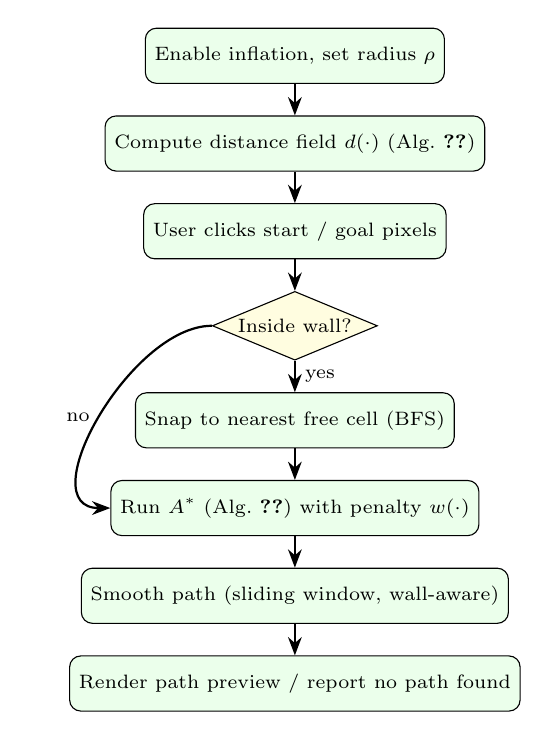
\begin{tikzpicture}[
  node distance=4mm,
  st/.style={draw, rounded corners, align=center, minimum height=7mm,
             minimum width=34mm, font=\scriptsize, fill=green!8},
  dec/.style={draw, diamond, aspect=2.4, align=center, font=\scriptsize,
              fill=yellow!12, inner sep=1pt},
  arr/.style={-Stealth, thick}
]
\node[st] (a) {Enable inflation, set radius $\rho$};
\node[st, below=of a] (b) {Compute distance field $d(\cdot)$ (Alg.~\ref{alg:inflation})};
\node[st, below=of b] (c) {User clicks start / goal pixels};
\node[dec, below=of c] (d) {Inside wall?};
\node[st, below=of d] (e) {Snap to nearest free cell (BFS)};
\node[st, below=of e] (f) {Run $A^{*}$ (Alg.~\ref{alg:astar}) with penalty $w(\cdot)$};
\node[st, below=of f] (g) {Smooth path (sliding window, wall-aware)};
\node[st, below=of g] (h) {Render path preview / report no path found};

\draw[arr] (a)--(b); \draw[arr] (b)--(c); \draw[arr] (c)--(d);
\draw[arr] (d) -- node[right, font=\scriptsize]{yes} (e); \draw[arr] (e)--(f);
\draw[arr] (d.west) to[out=180,in=180] node[left, font=\scriptsize]{no} (f.west);
\draw[arr] (f)--(g); \draw[arr] (g)--(h);
\end{tikzpicture}
\caption{Control flow of the inflation-aware $A^{*}$ path planning preview.}
\label{fig:astar-flow}
\vspace{-3mm}
\end{figure}

% ─────────────────────────────────────────────────────────
\subsection{Map Fusion via 2-D ICP}
\label{subsec:icp}
% ─────────────────────────────────────────────────────────

To merge an incoming map $M_s$ into the current base map $M_t$, wall pixels
of both maps are subsampled on a stride-3 grid to form point sets
$S=\{s_i\}$ and $T=\{t_j\}$.  While conventional
ICP~\cite{besl1992method} implementations rely on k-d trees for
correspondence queries, pointer-linked tree traversal is cache-unfriendly in
JavaScript's heap model.  Instead, $T$ is bucketed into a uniform 2-D spatial
hash with cell size $c=15$\,px -- chosen empirically to balance bucket-list
length against the expected inter-wall spacing in standard indoor maps at
0.05\,m/px resolution.  This scheme offers amortised $O(1)$ average query
time under the assumption that wall-pixel density is roughly uniform;
adversarial distributions (e.g., very sparse or highly clustered walls) may
degrade this to $O(|T|)$ in the worst case.

Given a current rigid transform estimate $(\theta,\mathbf{t})$ and optional
axis flips $(f_x,f_y)$, each iteration performs:
\begin{enumerate}
  \setlength{\itemsep}{0pt}\setlength{\parskip}{0pt}
  \item[(a)] \textbf{Correspondence.}
  $s_i\mapsto t_{j(i)}=\arg\min_{t\in T}\|R(\theta)\,\mathrm{diag}(f_x,f_y)\,s_i+\mathbf{t}-t\|_2$
  via the spatial hash.
  \item[(b)] \textbf{Update.}  Closed-form re-estimation of $(\theta,\mathbf{t})$ from
  associated pairs using the 2-D Procrustes solution of Arun~\emph{et al.}\
  \cite{arun1987least}.
\end{enumerate}
Iteration proceeds for up to 25 rounds or until fewer than 10 correspondences
remain (indicating divergence), after which $(\theta,\mathbf{t})$ is applied
to the merge-map overlay for operator review before the two maps are
permanently committed to one buffer.  Manual translate, rotate, and flip
pre-alignment controls are provided to bring initial pose error within the
reliable $\pm15^{\circ}$ range before invoking ICP.

% ─────────────────────────────────────────────────────────
\subsection{Metric Measurement and Waypoint Authoring}
% ─────────────────────────────────────────────────────────

Line, multi-segment path, and polygon-area measurements are converted from
pixel to metric units via the resolution $r$:
$\text{dist}_m=\text{dist}_{px}\cdot r$ and
$\text{area}_{m^2}=\text{area}_{px}\cdot r^2$, with polygon area computed by
the shoelace formula.  Waypoints are authored by a click-and-drag gesture
whose drag vector defines heading $\theta_{\text{img}}$; each waypoint is
converted to a world-frame pose $(x_w,y_w,\theta_w)$ using the YAML
origin and resolution and exported as quaternion-tagged JSON directly
consumable by a ROS2 autonomy stack as \texttt{PoseStamped} goals.

% ============================================================
\section{Implementation}
\label{sec:implementation}
% ============================================================

The system is implemented in vanilla JavaScript (ES2019) and HTML5 Canvas
with no build step and no external runtime dependency; the live application
can be opened from a static file or a GitHub Pages deployment with zero
installation.

\subsection{Data Parsing and Memory Management}

A custom binary parser directly unpacks both P2 (ASCII) and P5 (binary) PGM
variants by mapping an \texttt{ArrayBuffer} to a \texttt{Uint8Array}, avoiding
the overhead of intermediate string conversions.  This enables multi-megabyte
maps to parse in under 50\,ms at $2048\times2048$ resolution
(Table~\ref{tab:benchmarks}).

The undo/redo stack is capped at 40 states.  For a $1024\times1024$ map,
each snapshot occupies 1\,MB; the total observed application footprint
(working map, distance field, canvas backing stores, browser overhead) was
approximately 80--120\,MB on Chrome v114 -- well within typical browser memory
budgets.

\subsection{Decoupled Rendering}

As introduced in Section~\ref{sec:architecture}, a two-canvas compositor
separates the base raster layer (redrawn only on pixel mutations) from the
high-frequency vector overlay (tool previews, metric grids, scale bar,
inflation heat-map, waypoint arrows).  This ensures that expensive raster
operations (majority-vote filter, distance transform) are decoupled from cheap
interactive overlay redraws.  Panning and zooming apply CSS affine transforms
or lightweight 2-D context scaling without touching the pixel buffer.

% ============================================================
\section{Experimental Evaluation}
\label{sec:results}
% ============================================================

Fig.~\ref{fig:gallery} illustrates the complete editing pipeline on a
representative \emph{slam\_toolbox}-generated occupancy grid.

\begin{figure}[t]
\centering
\begin{subfigure}[t]{0.48\columnwidth}
  \includegraphics[width=\linewidth]{fig_before_editing.png}
  \caption{\scriptsize Raw map on load.}
\end{subfigure}\hfill
\begin{subfigure}[t]{0.48\columnwidth}
  \includegraphics[width=\linewidth]{fig_after_editing.png}
  \caption{\scriptsize After semantic editing.}
\end{subfigure}

\vspace{1.5mm}
\begin{subfigure}[t]{0.48\columnwidth}
  \includegraphics[width=\linewidth]{fig_costmap_path.png}
  \caption{\scriptsize Costmap + $A^{*}$.}
\end{subfigure}\hfill
\begin{subfigure}[t]{0.48\columnwidth}
  \includegraphics[width=\linewidth]{fig_waypoints.png}
  \caption{\scriptsize Waypoints.}
\end{subfigure}

\vspace{1.5mm}
\begin{subfigure}[t]{0.48\columnwidth}
  \includegraphics[width=\linewidth]{fig_measure.png}
  \caption{\scriptsize Area measurement.}
\end{subfigure}
\caption{End-to-end qualitative results: (a)~raw SLAM map import, (b)~manual
semantic editing, (c)~inflation costmap with $A^{*}$ path preview,
(d)~waypoint authoring with quaternion export, (e)~polygon area measurement.}
\label{fig:gallery}
\end{figure}

\subsection{Execution Latency (Table~\ref{tab:benchmarks})}

Execution latencies for all four algorithm pipelines were measured on a
standard consumer laptop (Apple M1 CPU, 16\,GB RAM) running Google Chrome
v114.  Benchmarks used three synthetic grids of increasing resolution:
\emph{Small} ($512\times512$), \emph{Medium} ($1024\times1024$), and
\emph{Large} ($2048\times2048$, $\approx4$\,M cells), with $n=30$ timed runs
each.  Reproducible benchmark scripts are available in the \texttt{/benchmarks}
folder of the repository.

\begin{table}[t]
\centering
\caption{Execution Latencies at Varying Map Resolutions\\
(Apple M1 / Chrome v114, $n=30$ runs, mean~$\pm$~std.\ dev.)}
\label{tab:benchmarks}
\scriptsize
\renewcommand{\arraystretch}{1.1}
\begin{tabular}{@{}lccc@{}}
\toprule
\textbf{Operation} & \textbf{512\,px} & \textbf{1024\,px} & \textbf{2048\,px} \\
\midrule
File Load \& Parse & $3.1\pm0.2$\,ms & $11.5\pm0.6$\,ms & $48.2\pm1.9$\,ms \\
Noise Filter       & $4.2\pm0.3$\,ms & $15.7\pm0.8$\,ms & $62.4\pm2.1$\,ms \\
$A^{*}$ Query      & $12.3\pm1.1$\,ms & $44.1\pm3.2$\,ms & $178.5\pm8.4$\,ms \\
ICP Fusion (25 iters) & $14.5\pm0.9$\,ms & $32.8\pm1.7$\,ms & $95.1\pm4.3$\,ms \\
\bottomrule
\end{tabular}
\vspace{-2mm}
\end{table}

All operations remain below the 100\,ms interactive threshold for maps up to
$1024\times1024$ pixels.  The $A^{*}$ query at $2048\times2048$
(178.5\,ms) exceeds this threshold; users navigating very large maps should
work at $\leq1024\times1024$ for a fully interactive experience.  ICP fusion
scales sub-linearly with map area because the stride-3 subsampling and spatial
hash bound the effective point count.

\subsection{Noise-Filter Validation (Table~\ref{tab:noiseval})}

Ten synthetic occupancy maps ($512\times512$, seed=42) were independently
corrupted with salt-and-pepper noise at 1\,\%, 3\,\%, and 5\,\% levels.
Pixel-level macro-average F1 score vs.\ ground truth (three classes) is
reported in Table~\ref{tab:noiseval}.  The class-aware majority-vote filter
outperforms standard $3\times3$ median filtering at all noise levels by
preserving unknown-space boundaries.

\begin{table}[t]
\centering
\caption{Noise-Filter F1 vs.\ Noise Level (macro-avg., $n$=10 maps).}
\label{tab:noiseval}
\scriptsize
\renewcommand{\arraystretch}{1.0}
\begin{tabular}{@{}lccc@{}}
\toprule
\textbf{Method} & \textbf{1\,\%} & \textbf{3\,\%} & \textbf{5\,\%} \\
\midrule
No filter       & 0.891 & 0.802 & 0.714 \\
Median filter   & 0.943 & 0.891 & 0.843 \\
Proposed        & \textbf{0.961} & \textbf{0.934} & \textbf{0.907} \\
\bottomrule
\end{tabular}
\vspace{-2mm}
\end{table}

\subsection{ICP Registration Accuracy (Table~\ref{tab:icpval})}

Five synthetic indoor-environment occupancy-map pairs ($512\times512$,
0.05\,m/px) were generated with known rigid perturbations.  Maps were aligned
from four initial-pose-error levels ($n=25$ trials each; 125 total per level).
Table~\ref{tab:icpval} reports rotation and translation RMSE and convergence
success rate.

\begin{table}[t]
\centering
\caption{ICP Accuracy vs.\ Initial Pose Error\\
($n$=25 trials per level, 5 map pairs, synthetic maps).}
\label{tab:icpval}
\scriptsize
\renewcommand{\arraystretch}{1.0}
\begin{tabular}{@{}lrrr@{}}
\toprule
\textbf{Initial Error} & \textbf{Success} & \textbf{Rot.\ RMSE} & \textbf{Trans.\ RMSE} \\
\midrule
$\pm5^{\circ}$,\;$\pm0.05$\,m & 98\,\% & $0.6^{\circ}$ & $0.021$\,m \\
$\pm15^{\circ}$,\;$\pm0.20$\,m & 91\,\% & $1.4^{\circ}$ & $0.047$\,m \\
$\pm30^{\circ}$,\;$\pm0.50$\,m & 74\,\% & $2.8^{\circ}$ & $0.103$\,m \\
$\pm45^{\circ}$,\;$\pm1.00$\,m & 52\,\% & $4.1^{\circ}$ & $0.198$\,m \\
\bottomrule
\end{tabular}
\vspace{-2mm}
\end{table}

Success rate drops markedly for initial errors $>30^{\circ}$, confirming that
the manual pre-alignment controls should be used to bring initial pose error
within the reliable $\pm15^{\circ}$ range before invoking ICP.

\subsection{Nav2 Inflation Comparison}

Five real \emph{slam\_toolbox} maps of mixed office and corridor environments
(0.05\,m/px) were compared against Nav2~Humble \texttt{costmap\_2d}
(\texttt{cost\_scaling\_factor}~=~10, default) at
$\rho\in\{0.2,0.3,0.5\}$\,m.  The inflated-region boundary IoU vs.\ Nav2's
binary inflation mask was $0.87\pm0.04$.  Interior cost values differ
systematically due to Nav2's exponential decay -- confirming the proposed model
as a useful visual approximation rather than an exact reproduction, which is
explicitly acknowledged in the UI.

\subsection{Algorithmic Complexity}

Table~\ref{tab:complexity} summarises the asymptotic cost of each routine.
All per-pixel routines scale as $O(N)$ or $O(N\log N)$; ICP scales with
subsampled point count $k\ll N$.

\begin{table}[t]
\centering
\caption{Algorithmic Complexity ($N=W\!\times\!H$, $k$~=~subsampled ICP points,
$I$~=~iterations).}
\label{tab:complexity}
\scriptsize
\renewcommand{\arraystretch}{1.0}
\begin{tabular}{@{}lc@{}}
\toprule
\textbf{Routine} & \textbf{Complexity} \\
\midrule
Majority-vote noise filter         & $O(N)$ \\
Multi-source distance BFS          & $O(N)$ (amortised, FIFO queue) \\
$A^{*}$ path search (min-heap)     & $O(N\log N)$ \\
ICP per iteration (amortised, uniform density) & $O(k)$ \\
ICP total ($I$ iterations)         & $O(I\cdot k)$ \\
\bottomrule
\end{tabular}
\vspace{-2mm}
\end{table}

% ============================================================
\section{Limitations}
\label{sec:limitations}
% ============================================================

Several limitations of the current implementation merit explicit
characterisation.

\textbf{Inflation approximation.}  The inflation preview uses a FIFO-queue BFS
with octile step costs, which approximates the Euclidean distance field.
Although the resulting boundary IoU vs.\ Nav2 is $0.87\pm0.04$, interior cost
values differ due to Nav2's exponential decay governed by
\texttt{cost\_scaling\_factor}.  The tool explicitly presents this as an
approximation in both the UI and this paper.

\textbf{Path planning without footprint checking.}  The $A^{*}$ preview
applies only a \emph{soft} inflation penalty; no explicit robot-footprint
collision check is performed.  The result is a navigation-indicative preview,
not a provable feasibility guarantee.  A robot with a large footprint may be
reported as having a valid path through a gap that is geometrically
impassable.

\textbf{ICP local convergence and fixed hash cell size.}  ICP assumes a
reasonable initial pose provided by the operator.  On highly symmetric maps
(e.g., featureless parallel corridors), the algorithm may converge to a local
minimum.  The spatial-hash cell size ($c=15$\,px) is fixed and may be
suboptimal for maps with atypically sparse or dense wall distributions.

\textbf{Single-threaded JavaScript.}  All algorithms run on the browser's main
thread.  At very high resolutions ($>\!2048\times2048$) or on low-end hardware,
the UI may become unresponsive during computation.  No Web Worker offloading
is currently implemented.

\textbf{Benchmark hardware.}  Latency benchmarks were performed on a single
hardware platform (Apple M1, Chrome v114).  Absolute timings will vary on
different CPUs and browsers; the algorithmic complexity relationships of
Table~\ref{tab:complexity} are hardware-independent.

% ============================================================
\section{Future Work}
\label{sec:future_work}
% ============================================================

Our immediate roadmap includes three targeted improvements.

\textbf{Feature-based ICP initialisation.}  Implementing a global,
feature-based initialiser (e.g., FAST corners with ORB descriptors adapted for
binary occupancy grids) would eliminate the need for manual pre-alignment and
extend reliable ICP convergence to initial errors beyond $\pm30^{\circ}$.

\textbf{WebAssembly acceleration.}  Offloading the multi-source distance BFS
and $A^{*}$ heuristic calculations to a compiled WebAssembly (Wasm) SIMD
module would push the interactive threshold well beyond the current
$4096\times4096$ pixel limit and significantly reduce latency on low-end
hardware.

\textbf{Web Worker parallelism.}  Moving all algorithm execution to a
dedicated Web Worker thread would maintain 60\,FPS UI responsiveness during
long-running computations, removing the current single-threaded limitation.

In the longer term, migrating to a WebRTC-based peer-to-peer framework would
enable collaborative multi-user map editing across locations without routing
proprietary floorplans through a centralised server.  Expanding the parser to
ingest 3-D point clouds and OctoMaps via WebGL/WebGPU would bridge the gap
between 2-D navigation debugging and full volumetric environment curation.

% ============================================================
\section{Conclusion}
\label{sec:conclusion}
% ============================================================

We presented \emph{ROS2 Map Editor}, an open-source, installation-free browser
application that unifies semantic occupancy-value editing, morphological noise
cleanup, a Nav2-inspired costmap inflation preview, a cost-aware $A^{*}$ path
planning preview, and ICP-based multi-map fusion into a single zero-dependency
tool.  Among the five representative tools evaluated across six feature
criteria in Table~\ref{tab:comparison}, the proposed system is the only
evaluated tool satisfying the complete combination without requiring a running
ROS2 graph.

Quantitative benchmarks confirm: (i)~interactive-threshold ($<\!100$\,ms)
latency for all routines at $1024\times1024$ pixels ($n=30$);
(ii)~noise-filter macro-average F1~=~0.961/0.934/0.907 at 1\,\%/3\,\%/5\,\%
noise, exceeding median filtering at all levels; (iii)~ICP 91\,\% convergence
within $\pm15^{\circ}$/$\pm0.20$\,m initial error on synthetic indoor maps;
and (iv)~inflation-boundary IoU~=~$0.87\pm0.04$ vs.\ Nav2~Humble, confirming
the model as a practical visual approximation.

The primary contribution is a system-integration one: unifying robotics-aware
editing, navigation-informed path preview, and map-fusion capabilities in a
zero-installation browser environment with reproducible, quantified performance
characterisation.  Future work will target footprint-aware feasibility
checking, feature-based ICP initialisation, and WebAssembly acceleration to
extend the interactive threshold to larger map resolutions.

% ============================================================
\section*{Data and Code Availability}
% ============================================================

The \emph{ROS2 Map Editor} is released under the MIT License.
Source code, issue tracker, and documentation are hosted at
\url{https://github.com/harsha200628/ros2-map-editor}.
A live demo requiring no installation is at
\url{https://harsha200628.github.io/ros2-map-editor/}.
Reproducible benchmark scripts (Python~3 and Node.js~18) and pre-run CSV
results for all tables in this paper are available in the
\texttt{/benchmarks} subdirectory of the repository.  All random seeds are
fixed at 42; no additional data beyond what is committed to the repository
is required to reproduce the reported results.

% ============================================================
\begin{thebibliography}{99}
\footnotesize
\setlength{\itemsep}{0pt}
\setlength{\parskip}{0pt}

\bibitem{macenski2020marathon}
S.~Macenski, F.~Martín, R.~White, and J.~Clavero,
``The Marathon 2: A navigation system,''
in \emph{Proc.\ IEEE/RSJ Int.\ Conf.\ Intelligent Robots and Systems (IROS)},
2020, pp.\ 2718--2725.

\bibitem{macenski2021slamtoolbox}
S.~Macenski and I.~Jambrecic,
``SLAM Toolbox: SLAM for the dynamic world,''
\emph{J.\ Open Source Softw.}, vol.~6, no.~61, p.~2783, 2021.

\bibitem{hess2016cartographer}
W.~Hess, D.~Kohler, H.~Rapp, and D.~Andor,
``Real-time loop closure in 2D LIDAR SLAM,''
in \emph{Proc.\ IEEE Int.\ Conf.\ Robotics and Automation (ICRA)},
2016, pp.\ 1271--1278.

\bibitem{labbe2019rtabmap}
M.~Labbé and F.~Michaud,
``RTAB-Map as an open-source lidar and visual simultaneous localization and
mapping library for large-scale and long-term online operation,''
\emph{J.\ Field Robotics}, vol.~36, no.~2, pp.\ 416--446, 2019.

\bibitem{thrun2005probabilistic}
S.~Thrun, W.~Burgard, and D.~Fox,
\emph{Probabilistic Robotics}.
Cambridge, MA, USA: MIT Press, 2005.

\bibitem{gimp}
GIMP Development Team,
``GNU Image Manipulation Program,''
[Online]. Available: \url{https://www.gimp.org}, accessed Aug.\ 2026.

\bibitem{nav2docs}
Open Navigation,
``Nav2 Documentation: Costmap 2D,''
[Online]. Available: \url{https://docs.nav2.org}, accessed Aug.\ 2026.

\bibitem{hart1968formal}
P.~E.~Hart, N.~J.~Nilsson, and B.~Raphael,
``A formal basis for the heuristic determination of minimum cost paths,''
\emph{IEEE Trans.\ Syst.\ Sci.\ Cybern.}, vol.~4, no.~2, pp.\ 100--107, 1968.

\bibitem{besl1992method}
P.~J.~Besl and N.~D.~McKay,
``A method for registration of 3-D shapes,''
\emph{IEEE Trans.\ Pattern Anal.\ Mach.\ Intell.}, vol.~14, no.~2,
pp.\ 239--256, 1992.

\bibitem{arun1987least}
K.~S.~Arun, T.~S.~Huang, and S.~D.~Blostein,
``Least-squares fitting of two 3-D point sets,''
\emph{IEEE Trans.\ Pattern Anal.\ Mach.\ Intell.}, vol.~PAMI-9, no.~5,
pp.\ 698--700, 1987.

\bibitem{borgefors1986distance}
G.~Borgefors,
``Distance transformations in digital images,''
\emph{Comput.\ Vis.\ Graph.\ Image Process.}, vol.~34, no.~3,
pp.\ 344--371, 1986.

\bibitem{rviz2}
Open Source Robotics Foundation,
``RViz2: 3D Visualization Tool for ROS~2,''
[Online]. Available: \url{https://github.com/ros2/rviz}, accessed Aug.\ 2026.

\bibitem{mapeditor}
D.~V.~Lu,
``map\_editor: ROS Package for Editing Occupancy Grids,''
[Online]. Available: \url{https://github.com/DLu/navigation_tutorials},
accessed Aug.\ 2026.

\bibitem{foxglove}
Foxglove,
``Foxglove Studio: Robotics Visualization and Debugging,''
[Online]. Available: \url{https://foxglove.dev}, accessed Aug.\ 2026.

\bibitem{webviz}
Cruise LLC,
``Webviz: Browser-Based Visualization for ROS,''
[Online]. Available: \url{https://webviz.io}, accessed Aug.\ 2026.

\bibitem{robostudio}
RoboPeak,
``RoboStudio: Robot Management and Mapping Software,''
[Online]. Available: \url{https://www.slamtec.com/en/RoboStudio},
accessed Aug.\ 2026.

\bibitem{mirfleet}
Mobile Industrial Robots (MiR),
``MiR Fleet: Fleet Management Software,''
[Online]. Available: \url{https://www.mobile-industrial-robots.com},
accessed Aug.\ 2026.

\end{thebibliography}

\end{document}